\chapter{Grafi}

{Coppia ordinata $G=(V,E)$ formata da due insiemi $V$ (vertici) ed $E$ (archi)}

$V = \{1,2,3,\ldots,n\}$

{$E \subseteq VxV$, ovvero $E$ è un sottoinsieme dell'insieme delle parti (prodotto cartesiano) dell'insieme $V$}

{I grafi possono essere}

\begin{itemize}
\tightlist
\item
  {Orientati}
\item
  {Non orientati, se le relazioni sono simmetriche}
\end{itemize}

{~~~~~~~~se $\forall(u,v) \in E \iff (v,u) \in E$}

{Non si ammettono cappi nei grafi non orientati.}

$\forall u \in E \iff (u,u) \notin E$

\section{Sottografi}

{Sottografo di $G$}

{$G'=(V',E')$ è sottografo di $G$ se $V'\subseteq V$ e $E'\subseteq E$}

\paragraph{Sottografo indotto}

{Dato $V' \subseteq V$, il sottografo indotto da $V'$ di $G$ è $G[V']=(V',E')$, con $E' = E\,\cap\,V\,x\,V'$}

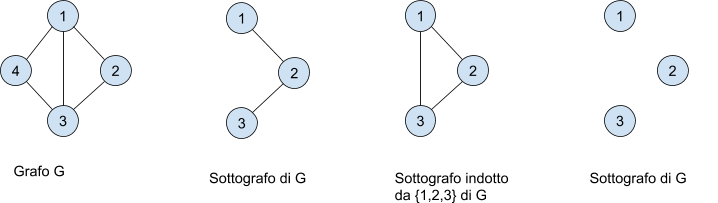
\includegraphics{images/image534.png}

\section{Cammini}

{Un cammino di $G$ è una sequenza $<X_0,X_1,\ldots,X_k>$ dove i vertici appartengono al grafo di partenza.}

$\forall i,0\leq i\leq k,(X_i,X_{i+1})\in E$

\subsection{Cammini semplici e cammini non semplici}

$<1,2,3,4,5>$ è un cammino semplice\\
$<1,2,3,1,4,5>$ non è un cammino semplice

{Un cammino è semplice se tutti i vertici sono distinti}

\paragraph{Lunghezza di un cammino}

{La lunghezza di un cammino è il numero dei suoi archi}

\paragraph{Raggiungibilità dei vertici}

$u$ è raggiungibile da $v$ se esiste un cammino $<X_0,X_1,X_2,\ldots,X_k>$ tale che $X_0 = u$ e $X_k = v$

\paragraph{Ciclo}

{Un ciclo è un cammino dove $X_0 = X_k$}

{Un grafo senza cicli si dice aciclico.}

\paragraph{{[}NO{]}Grafo connesso}

{Un grado non orientato si dice connesso se $\forall (u,v) | u,v \in V$, esiste un cammino da $u$ a $v$ con $u\neq v$}

\paragraph{{[}NO{]} Componente connessa}

{Dato $G=(V,E)$ e $V' \subseteq V$}

{$V'$ si dirà componente connessa se }

\begin{enumerate}
\tightlist
\item
  {$G[V']$ è connesso}
\item
  $V'${~non è sottoinsieme stretto di un sottografo connesso}
\end{enumerate}

{Se il numero di componenti connesse di un grafo è uguale a 1, }{il
grafo è connesso.}

\paragraph{{[}NO{]}Vertici adiacenti}

{Dato $G=(V,E)$ e $u \in V$}

{Il grado di $u$, $deg(u)$ è il numero di vertici adiacenti a $u$}

\paragraph{Arco incidente}

{Un arco che è collegato ad $v$}

\paragraph{Vertici isolati e terminali}

{Se $deg(u) = 0$ allora $u$ è isolato}

{Se $deg(u) = 1$ allora $u$ è terminale}

\section{Teorema della stretta di mano (HandShaking Lemma)}

{{[}NO{]}}

\begin{equation}
\sum_{u \in V}{degree(u)} = 2m
\end{equation}

{dove $m = \abs{E}$ è il numero di archi.}

{{[}O{]}}

{$outDegree(u)$ : numero degli archi uscenti da $u$}

{$inDegree(u)$ : numero degli archi entranti in $u$}

\begin{equation}
\sum_{u \in V}{outDegree(u)} = \sum_{u \in V}{inDegree(u)} = m
\end{equation}

{{[}NO{]} Proprietà}

{Il numero di vertici che hanno grado dispari è sempre pari}

\paragraph{Dimostrazione}

$V=P\cup D$

$P = \{u \in V | deg(u) \, pari\}$

$D = \{u \in V | deg(u) \, dispari\}$

$2m = \sum_{u \in V}{deg(u)} = \sum_{u \in P}{deg(u)} + \sum_{u \in D}{deg(u)}$

$2m = \sum_{u \in P}{2*h(u)} + \sum_{u \in D}{2*h(u)+1}$

$2m = \sum_{u \in P}{2*h(u)} + \sum_{u \in D}{2*h(u)} + \abs{D}$

$\abs{D} = 2m - 2 *\sum_{u \in P}{h(u)} + 2*\sum_{u \in D}{h(u)}$

$\abs{D} = 2*(m-\sum_{u \in V}{h(u)})$

{Il numero di vertici con grado dispari è quindi pari}

\paragraph{Esercizio}
{~~~~~~~~Dimostrare che, dato $G=(V,E)$ non orientato senza vertici isolati (nessuno vertice ha grado 0),}

{~~~~~~~~con $\abs{E} = \abs{V} -1$}

{Allora, esistono almeno due vertici terminali}

{Dimostrazione per assurdo:}

$n=\abs{V},m=\abs{E}$

{Per il lemma della stretta di mano:}

$\sum_{u \in V}{deg(u)} = 2$ e $\abs{E} = 2m$

$2n-2 = 2m = \sum_{u \in V}{deg(u)}$

{Chiamo $V_1$ un sottoinsieme di $V$ di vertici terminali}

$V_1=\{u\in V\,|\,deg(u)=1\}$

{Il problema diventa: dimostrare che $\abs{V_1} \geq 2$}

$2m = \sum_{u \in V_1}{deg(u)} +  \sum_{u \in V \setminus V_1}{deg(u)}$

$2n -2 \geq 2n - \abs{V_1}$

{????}\textsuperscript{\protect\hyperlink{cmnt21}{{[}u{]}}}

{$\abs{V_1} \geq 2$ OK}

\section{Matrice di adiacenza}

{Dato $G=(V,E)$}

$n=\abs{V},m=\abs{E}$

{$A$ Matrice quadrata $n x n$ }

\begin{itemize}
\tightlist
\item
  {Per trovare il grado di un vertice basta calcolare la somma degli elementi sulla corrispondente riga}
\item
  {{[}NO{]} $n$ archi in totale = doppia somma di tutti gli elementi della matrice}
\item
  {{[}O{]} $n$ archi in totale = doppia somma di tutti gli elementi della matrice}
\end{itemize}

{Usare le matrici di adiacenza solitamente conviene se ci sono molti archi, altrimenti è meglio utilizzare le liste.}

\paragraph{Matrice di adiacenza per grafi orientati}

\begin{equation}
A_{i,j} = 
\begin{cases}
0 & \mbox{se } (i,j) \notin E \\ 
1 & \mbox{se } (i,j) \in E
\end{cases}
\end{equation}

{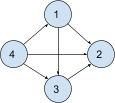
\includegraphics{images/image529.png}}

\begin{tabular}{|c|c|c|c|c|}
\hline 
  & \textbf{1} & \textbf{2} & \textbf{3} & \textbf{4} \\ 
\hline 
\textbf{1} & 0 & 1 & 1 & 0 \\ 
\hline 
\textbf{2} & 0 & 0 & 0 & 0 \\ 
\hline 
\textbf{3} & 0 & 1 & 0 & 0 \\ 
\hline 
\textbf{4} & 1 & 1 & 1 & 0 \\ 
\hline 
\end{tabular} 

\paragraph{Matrice di adiacenza per grafi non orientati}

\begin{equation}
A_{i,j} = 
\begin{cases}
0 & \mbox{se } \{i,j\} \notin E \\ 
1 & \mbox{se } \{i,j\} \in E
\end{cases}
\end{equation}

{Essendo la relazione tra vertici simmetrica, $A=A^T$ (trasposta)}

{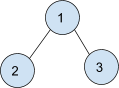
\includegraphics{images/image535.png}}

\begin{tabular}{|c|c|c|c|}
\hline 
  & \textbf{1} & \textbf{2} & \textbf{3} \\ 
\hline 
\textbf{1} & 0 & 1 & 1 \\ 
\hline 
\textbf{2} & 1 & 0 & 0 \\ 
\hline 
\textbf{3} & 1 & 0 & 0 \\ 
\hline 
\end{tabular} 

\section{Liste concatenate}

{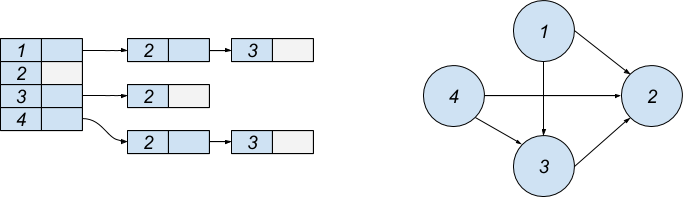
\includegraphics{images/image537.png}}

{Usare le liste di adiacenza solitamente conviene se ci sono pochi archi, altrimenti è meglio utilizzare le matrici.}

{{[}O{]} Densità}

\begin{equation}
\delta=\frac{numero\,di\,archi}{numero\,di\,possibili\,archi} = \frac{numero\,di\,archi}{n^2}
\end{equation}

$n=\abs{V},m=\abs{E}$

$\delta=\frac{m}{n^2}$

\paragraph{{[}NO{]} Densità}

\begin{equation}
\delta=\frac{numero\,di\,archi}{numero\,di\,possibili\,archi}
\end{equation}

{$\delta=\frac{m}{k},\,k = \frac{n(n-1)}{2}$ coefficiente binomiale}


{Grafi sparsi ($n\simeq m$): lista}

{Grafi densi ($n^2\simeq m$): matrice}

\paragraph{Proprietà}

{Sia $G$ un grafo NO. Se $G$ è aciclico, allora la cardinalità $\abs{E} \leq \abs{V}-1$}

\paragraph{ Dimostrazione induttiva su $n=\abs{V}$}

{~~~~~~~~Caso base:}

{~~~~~~~~~~~~~~~~se $n=1$ allora $m = 0$

{~~~~~~~~~~~~~~~~se $n=2$ allora $m \leq 1$

{~~~~~~~~Passo induttivo $n \geq 3$:}


\paragraph{{[}NO{]} Complemento di un grafo}

{Il complemento di un grafo è un grafo con gli stessi vertici, i cui archi sono complementari:}

$G=(V,E), \overline{G}=(\overline{V},\overline{E})$

\section{Grafo autocomplementare}

{Un grafo è detto autocomplementare se $\overline{G}=G$ ovvero se $\forall(i,j) \in E\,sse\,(i,j) \in \overline{E}$}

{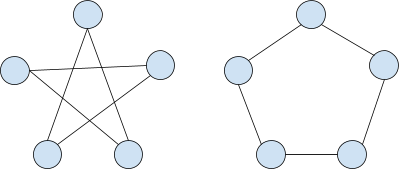
\includegraphics{images/image532.png}}

\subsection{Prodotto tra matrici di adiacenza}

\subsubsection{Prodotto di matrici}

{Due matrici $n\,x\,m$ ed $p\,x\,n$ (il numero di righe della prima equivale al numero di colonne della seconda) possono essere moltiplicate tramite il prodotto ``righe per colonne''.}

$C = A*B$ \\
$C_{i,j}=\sum_{k=1}^{n}{a_{i,k}*a_{k,j}}$

\subsubsection{Matrice al quadrato}


{Moltiplicando una matrice di adiacenza $A$ per se stessa, tramite il prodotto tra righe e colonne, ottengo una matrice delle stesse dimensioni con le seguenti caratteristiche:}

\begin{itemize}
\tightlist
\item
  {Sulla diagonale principale ho i gradi dei vertici}
\item
  {Nelle altre posizioni ho il numero di cammini tra i e j di lunghezza
  2}
\end{itemize}

$A^2 = A*A = (a^{(2)}_{i,j})$ \\
$a^{(2)}_{i,j}=\sum_{k=1}^{n}{a_{i,k}*a_{k,j}}$

\paragraph{Dimostrazione}

{``Sulla diagonale principale ho i gradi dei vertici'' ($i=j$)}

$a^{(2)}_{i,j}=\sum_{k=1}^{n}{a_{i,k}*a_{k,i}}$

{Essendo $G$ non orientato, la matrice è simmetrica e $a_{i,k}*a_{k,i} = a^2_{i,k}$}

{$a^{(2)}_{i,i} = \sum^n_{k=1}{a^2_{i,k}}$ , notiamo che il termine della sommatoria contiene solo valori binari che elevati al quadrato restituiscono il medesimo valore. Perciò}

$a^{(2)}_{i,i} = \sum^n_{k=1}{a^2_{i,k}} = \sum^n_{k=1}{a_{i,k}} = deg(i)$

{``Nelle altre posizioni ho il numero di cammini tra $i$ e $j$ di lunghezza'' ($i\neq j$)}

{$a^2_{i,j}=\sum_{k=1}^{n}{a_{i,k}*a_{k,j}}$, essendo la matrice di adiacenza composta da valori binari, il prodotto risulta valere 1 solo se entrambi i fattori valgono 1, ovvero se esiste un cammino di lunghezza 2}

\subsubsection{Matrice con esponente maggiore di 2}

{$A^n, n > 2$ conterrà}

\begin{itemize}
\tightlist
\item
  {Sulla diagonale: il numero di cicli di lunghezza n che partono da i}
\item
  {Fuori dalla diagonale: il numero di cammini di lunghezza n}
\end{itemize}

{Dimostrazione per induzione:}\textsuperscript{\protect\hyperlink{cmnt22}{{[}v{]}}\protect\hyperlink{cmnt23}{{[}w{]}}}

{Ipotesi:}

{~~~~~~~~Passo induttivo:}

$A^n = A *A* A * \ldots * A$ ($n$ volte) $=A^{n-1}*A$

{$a_{i,j^{(n)}} = \sum_{k=1}^n{a^{(n-1)}_{i,k}*a_{k,j}}$, ovvero il numero di cammini da $i$ a $j$ passanti per $k$.}

{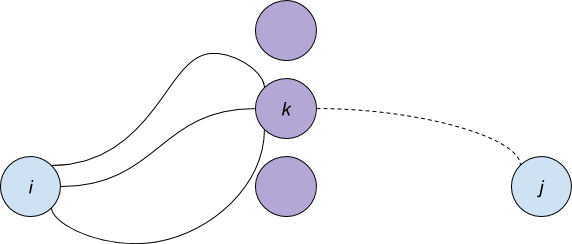
\includegraphics{images/image538.png}}

\paragraph{Esercizio}

{Mostrare che $G=(V,E) [NO]$ contiene un triangolo, ovvero un ciclo di lunghezza 3, se e solo se esistono due indici $i,j$ tali che sia la matrice di adiacenza $A$ e la matrice al quadrato $A^2$ hanno un elemento non nullo in posizione $(i,j)$}

\section{{[}NO{]} Grafi regolari}

{$G=(V,E)$ si dice k-regolare se tutti i vertici hanno grado $k$. Con $n=\abs{V},m=\abs{E}$}

{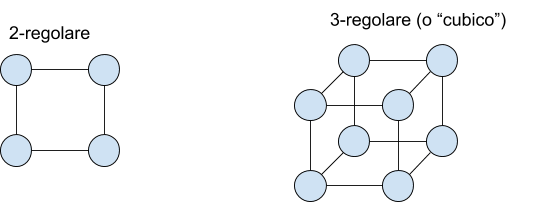
\includegraphics{images/image524.png}}

\paragraph{Proprietà}

{Se $G$ è 2-regolare allora il numero di vertici coincide necessariamente con il numero degli archi. $n=m$}

\paragraph{Dimostrazione}

{Utilizziamo il teorema della stretta di mano}

$2m=\sum_{u\in V}{deg(u)}$\textsuperscript{\protect\hyperlink{cmnt24}{{[}x{]}}\protect\hyperlink{cmnt25}{{[}y{]}}}

\paragraph{Esercizio}

{Dimostrare che se il grafo $G$ è 3-regolare, allora $n$ è pari. Analogamente, analizzare $G$ 4-regolare. }

\section{Isomorfismi di grafi}

{Un isomorfismo di grafi è un funzione che mappa un grafo in un secondo dalla stessa forma.}

{Viene fornita la definizione per i grafi non orientati, essa può però essere adattata a grafi orientati.}

\paragraph{{[}NO{]} Definizione}

$G_1=(v_1,E_1),G_2(V_2,E_2)$

{$\Theta:V_1\rightarrow V_2$ si dice isomorfismo se valgono le due proprietà:}

\begin{enumerate}
\tightlist
\item
  {$\Theta$ deve essere una funzione biettiva (è necessaria una corrispondenza 1-1).}
\item
  {La relazione di adiacenza deve essere preservata\\
  $\forall u,v \in V_1, (u,v) \in E_1 \iff (\Phi(u),\Phi(v)) \in E_2$}
\end{enumerate}

\subsection{Determinare se due grafi sono isomorfi}

{$G_1=(v_1,E_1),G_2(V_2,E_2)$ sono isomorfi se esiste un isomorfismo da $G_1$ a $G_2$ e si indica con $G_1\simeq G_2$}

{Condizioni necessarie perché $G_1\simeq G_2$:}

\begin{enumerate}
\tightlist
\item
  $\abs{V_1}=\abs{V_2}$
\item
  $\abs{E_1}=\abs{E_2}$
\item
  {Stessa degree sequence $degseq(G_1) = degseq(G_2)$}
\item
  $\#ComponentiConnesse(G_1) = 	\#ComponentiConnesse(G_2)$
\end{enumerate}


\begin{longtable}[]{@{}lll@{}}
\toprule
\begin{minipage}[t]{0.30\columnwidth}\raggedright\strut
$G$\strut
\end{minipage} & \begin{minipage}[t]{0.30\columnwidth}\raggedright\strut
$\overline{G}$\strut
\end{minipage} & \begin{minipage}[t]{0.30\columnwidth}\raggedright\strut
{Può verificarsi?}\strut
\end{minipage}\tabularnewline
\begin{minipage}[t]{0.30\columnwidth}\raggedright\strut
{Connesso}\strut
\end{minipage} & \begin{minipage}[t]{0.30\columnwidth}\raggedright\strut
{Connesso}\strut
\end{minipage} & \begin{minipage}[t]{0.30\columnwidth}\raggedright\strut
{FALSO}\strut
\end{minipage}\tabularnewline
\begin{minipage}[t]{0.30\columnwidth}\raggedright\strut
{Connesso}\strut
\end{minipage} & \begin{minipage}[t]{0.30\columnwidth}\raggedright\strut
{Disconnesso}\strut
\end{minipage} & \begin{minipage}[t]{0.30\columnwidth}\raggedright\strut
{FALSO \\ (Es: autocomplementare)}\strut
\end{minipage}\tabularnewline
\begin{minipage}[t]{0.30\columnwidth}\raggedright\strut
{Disconnesso}\strut
\end{minipage} & \begin{minipage}[t]{0.30\columnwidth}\raggedright\strut
{Connesso}\strut
\end{minipage} & \begin{minipage}[t]{0.30\columnwidth}\raggedright\strut
{VERO}\strut
\end{minipage}\tabularnewline
\begin{minipage}[t]{0.30\columnwidth}\raggedright\strut
{Disconnesso}\strut
\end{minipage} & \begin{minipage}[t]{0.30\columnwidth}\raggedright\strut
{Disconnesso}\strut
\end{minipage} & \begin{minipage}[t]{0.30\columnwidth}\raggedright\strut
{FALSO}\strut
\end{minipage}\tabularnewline
\bottomrule
\end{longtable}

{Il problema di determinare l'esistenza di un'isomorfismo tra due grafi è esoso in termini di tempo. Per evitare il bruteforce di tutte le combinazioni si procede a mappare gli archi con grado analogo.}

\section{Grafi planari}

Un grafo è planare se tutti archi non sono incidenti.

\begin{teorema}{Clique su grafi planari}{theoexample}
Le clique sui grafi planari hanno $k <= 4$. Con valori maggiori di 4 non è più possibile costruire clique su grafi planari.
\end{teorema}
